\documentclass[11pt, oneside]{article}          % use "amsart" instead of "article" for AMSLaTeX format
\usepackage[letterpaper,body={6.0in,8.0in},vmarginratio=1:1]{geometry}
\usepackage{graphicx}
\usepackage{caption}
\usepackage{subcaption}
\usepackage{amsmath}
\usepackage{todonotes}
\usepackage{booktabs}
\usepackage{comment}
\usepackage[hidelinks]{hyperref}

\usepackage{natbib}
\bibliographystyle{abbrvnat}
\setcitestyle{authoryear,open={},close={}}

\title{\vspace{-2.0cm}Compositional subgoal representations - Poster supplement}
\author{Carlos G. Correa}
\date{}

\begin{document}
\maketitle
%
%\begin{figure}[ht]
%  \centering
%  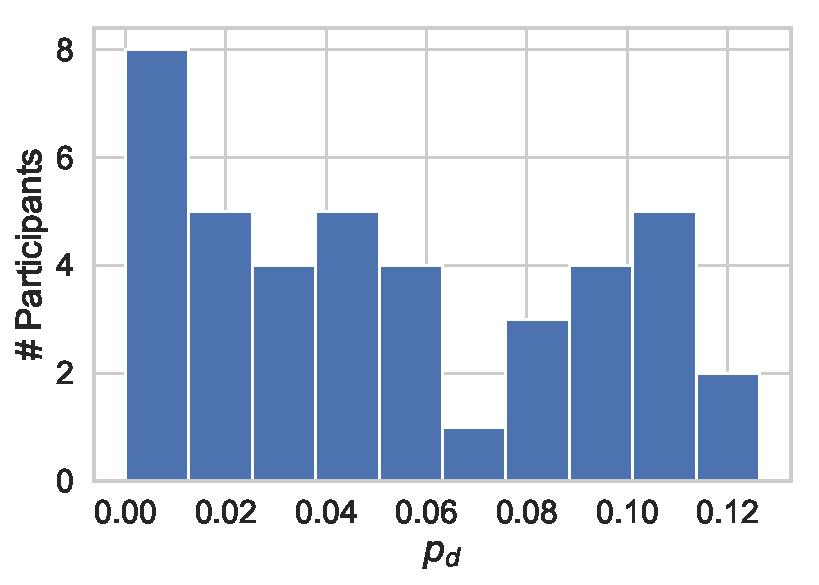
\includegraphics[width=0.45\textwidth]{geom-k-d}
%  \caption{Distribution of fit parameters for depth limits from best fitting Geometric $k$/$d$ model.}
%\end{figure}

\begin{figure}[ht]
  \centering
  \begin{subfigure}[t]{0.45\textwidth}
    \includegraphics[width=\textwidth]{geom-k-p}
    \caption{Distribution of fit parameters for multigoal size. Can be interpreted as probability of each participant using a multigoal with more than one subgoal for a single action. This probability is simply one minus the parameter of the Geometric distribution.}
  \end{subfigure}
  \hspace{1em} % here you can insert horizontal or vertical space
  \begin{subfigure}[t]{0.45\textwidth}
    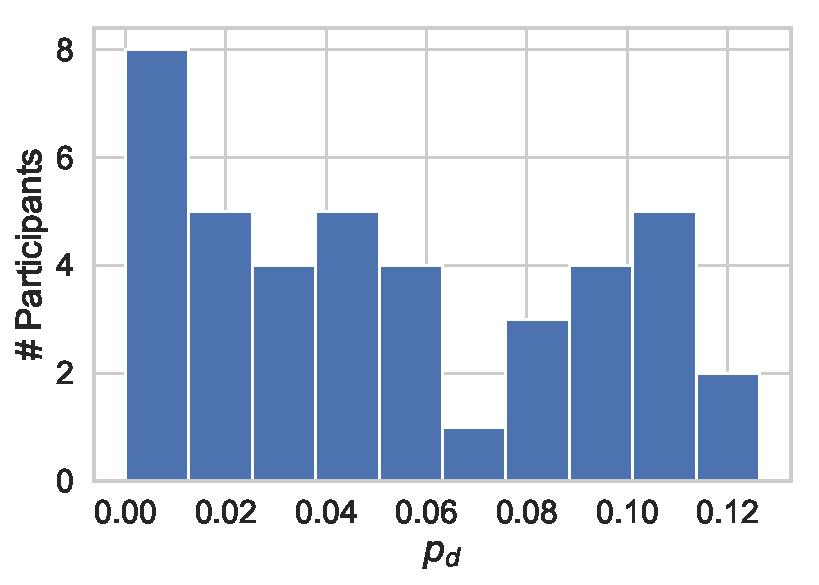
\includegraphics[width=\textwidth]{geom-k-d}
    \caption{Distribution of fit parameters for depth limits. Smaller numbers indicate larger expected values for depth limits.}
  \end{subfigure}
  \caption{Individual differences in parameters in best fitting Geometric $k$/$d$ model.}
  \label{fig:rpe}
\end{figure}


\begin{table}[ht!]
  \centering
  \begin{tabular}{lrrrrrrr}
  \toprule
  Model         & \# Params & AIC & BIC   & LL    & \# Best fit & $R^2$ & Trial Likelihood  \\
  \midrule
Geometric $k$/$d$ & 3 & \textbf{10293} & \textbf{10315} & -5143 & 6 & 0.709 & 63.69\% \\
Poisson $k$/$d$ & 3 & 10301 & 10323 & -5147 & 7 & 0.708 & 63.66\% \\
Poisson $k$ & 2 & 11074 & 11088 & -5535 & 2 & 0.686 & 61.72\% \\
Geometric $k$ & 2 & 11090 & 11104 & -5543 & 1 & 0.686 & 61.70\% \\
Fixed $k$/$d$ & 3 & 11278 & 11300 & -5636 & 0 & 0.681 & 61.17\% \\
Fixed $k$ & 2 & 11545 & 11560 & -5770 & 0 & 0.673 & 60.58\% \\
Poisson $d$ & 2 & 12204 & 12218 & -6100 & 9 & 0.655 & 57.88\% \\
$k$=1 & 1 & 12402 & 12410 & -6200 & 14 & 0.649 & 58.96\% \\
Geometric $d$ & 2 & 12902 & 12917 & -6449 & 2 & 0.635 & 55.98\% \\
Fixed $d$ & 2 & 13188 & 13203 & -6592 & 0 & 0.627 & 55.51\% \\
Random & 0 & 35312 & 35312 & -17656 & 0 & 0.000 & 19.93\% \\
  \bottomrule
  \end{tabular}
  \caption{Model comparison. Columns are number of parameters per participant, Akaike information criterion, Bayesian information criterion, log likelihood, the number of participants best fit by the model, McFadden's Pseudo-$R^2$, and the mean per-trial likelihood.}
  \label{tab:model-fits}
\end{table}



\end{document}
